\documentclass[11pt, oneside]{article}   	% use "amsart" instead of "article" for AMSLaTeX format
\usepackage{geometry}                		% See geometry.pdf to learn the layout options. There are lots.
\geometry{letterpaper}                   		% ... or a4paper or a5paper or ... 
%\geometry{landscape}                		% Activate for for rotated page geometry
%\usepackage[parfill]{parskip}    		% Activate to begin paragraphs with an empty line rather than an indent
\usepackage{graphicx}				% Use pdf, png, jpg, or eps� with pdflatex; use eps in DVI mode
								% TeX will automatically convert eps --> pdf in pdflatex		
\usepackage{amssymb}
\usepackage{amsmath}
\usepackage{parskip}
\usepackage{color}

\title{Proof for Ceva:  Lockhart}
%\author{The Author}
%\section{}
% \subsection*{R code}
\date{}							% Activate to display a given date or no date

\graphicspath{{/Users/telliott_admin/Dropbox/Tex/png/}}

% \begin{center} 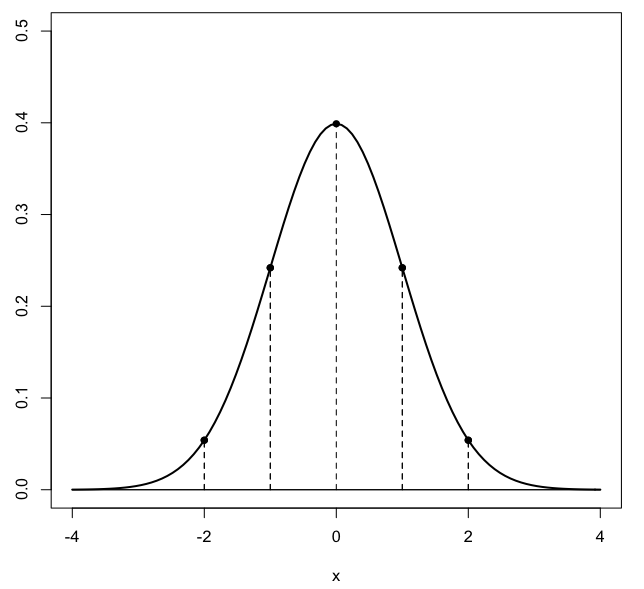
\includegraphics [scale=0.4] {gauss3.png} \end{center}

\begin{document}
\maketitle
\Large
\noindent

\begin{center} 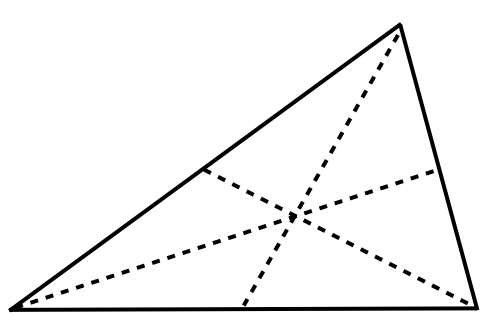
\includegraphics [scale=0.4] {ceva_small1.png} \end{center}

Ceva's Theorem says that if we start with a triangle and draw the line segments connecting each vertex with the midpoint of the opposite side, the three line segments cross at a single, unique point.  Furthermore, it is possible to show that for any of these line segments, this point (called the \emph{centroid}) lies one-third of the length from the side, and two-thirds of the length from the vertex.

In other write-ups I've shown one proof of this using similar triangles, and another using vectors.  This third approach is one outlined in Lockhart's book \emph{Measurement}.

\begin{center} 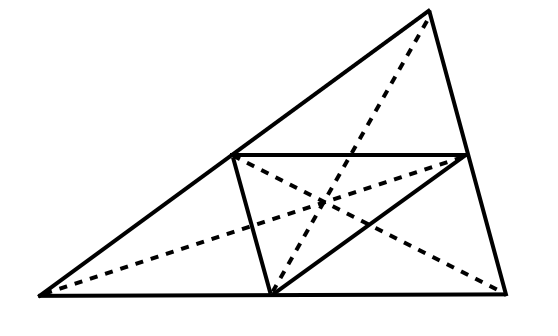
\includegraphics [scale=0.4] {ceva_small2.png} \end{center}

The idea is to connect the midpoints of the sides.  If we do that, the construction results in four smaller triangles.  It is easy to show that these triangles are congruent, and are similar to the large one we started with.  (By similar triangles, a short side opposite a midpoint/vertex is parallel to the side containing the midpoint.  I'm sure you can finish the proof).

Because of the congruent triangles, we also have three congruent parallelograms, and these have rotational symmetry around the centroid.

Therefore the centroid is a single point.

If you don't like that argument, notice that the dotted lines play the same role for each of the small triangles, extending from a vertex to the midpoint of the opposite side.  

What this means is that \emph{if} the centroid is a single point, then centroids of the larger triangle and the small central triangle are the same point.  But we can just continue in the same way, inscribing a new, even smaller, triangle, using the midpoints of the small central triangle, and this process can be extended \emph{ad infinitum}.  Hence, in the limit, we will reach a single point.

We can locate the centroid by imagining that we find successive midpoints of a length from opposite ends left and right.  The first point is at $1/2$ of the length (from the left), the second comes back from $1$ by $1/4$ so is at $0.75$ (at the right), the third is at $0.5 + 1/8$ (from the left), so every second round we get closer to the centroid  by advancing from the left by

\[ S = \frac{1}{2} +  \frac{1}{8} +  \frac{1}{32}  + \dots \]

Now, we can either assume this sum is finite (for now) or recognize that it is certainly smaller than 

\[ \frac{1}{2} +  \frac{1}{4} +  \frac{1}{8}  + \dots = 1 \]

\begin{center}
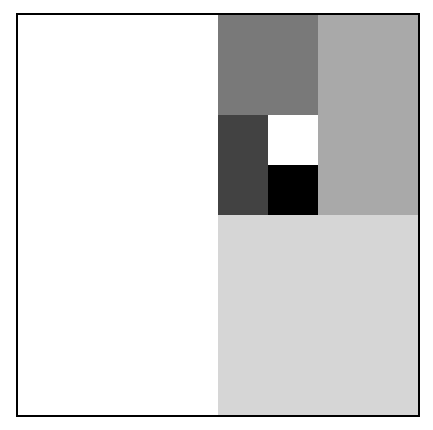
\includegraphics [scale=0.4] {series1.png}
\end{center}

So if
\[ S = \frac{1}{2} +  \frac{1}{8} +  \frac{1}{32}  + \dots \]
then
\[ 2S = 1 +  \frac{1}{4} +  \frac{1}{16}  + \dots \]
and
\[ 3S = 1S + 2S = 1 +  \frac{1}{2} +  \frac{1}{4} +  \frac{1}{8} + \frac{1}{16}   + \dots \]
That is, $3S = 1 + 1$, so $S = 2/3$.

\end{document}  